% =====================================================================
% Diagrama de casos de uso e esboço das telas --- Kaio (Frente 6)
% Só o Kaio edita este arquivo. Texto inicial montado a partir de
% documentos/uml/casos_de_uso.md (PR #5); o Kaio revisa e completa.
% =====================================================================
\section{Casos de uso e telas}\label{sec:casos}

A Figura~\ref{fig:casos} mostra os casos de uso da ferramenta. Há dois atores: o
\emph{usuário (analista)}, que opera a interface, e as \emph{bases de dados}, um sistema externo
que a ferramenta só lê. Os 17 casos de uso cobrem obter um grafo (carregando uma base real ou
gerando um grafo sintético), calcular métricas, detectar comunidades, identificar
influenciadores com a simulação SIR, visualizar a rede e ver ou exportar os resultados. A
descrição de cada caso de uso, com pré-condições e fluxos, está em
\codigo{documentos/uml/casos\_de\_uso.md}.

\begin{figure}[htbp]
\centering
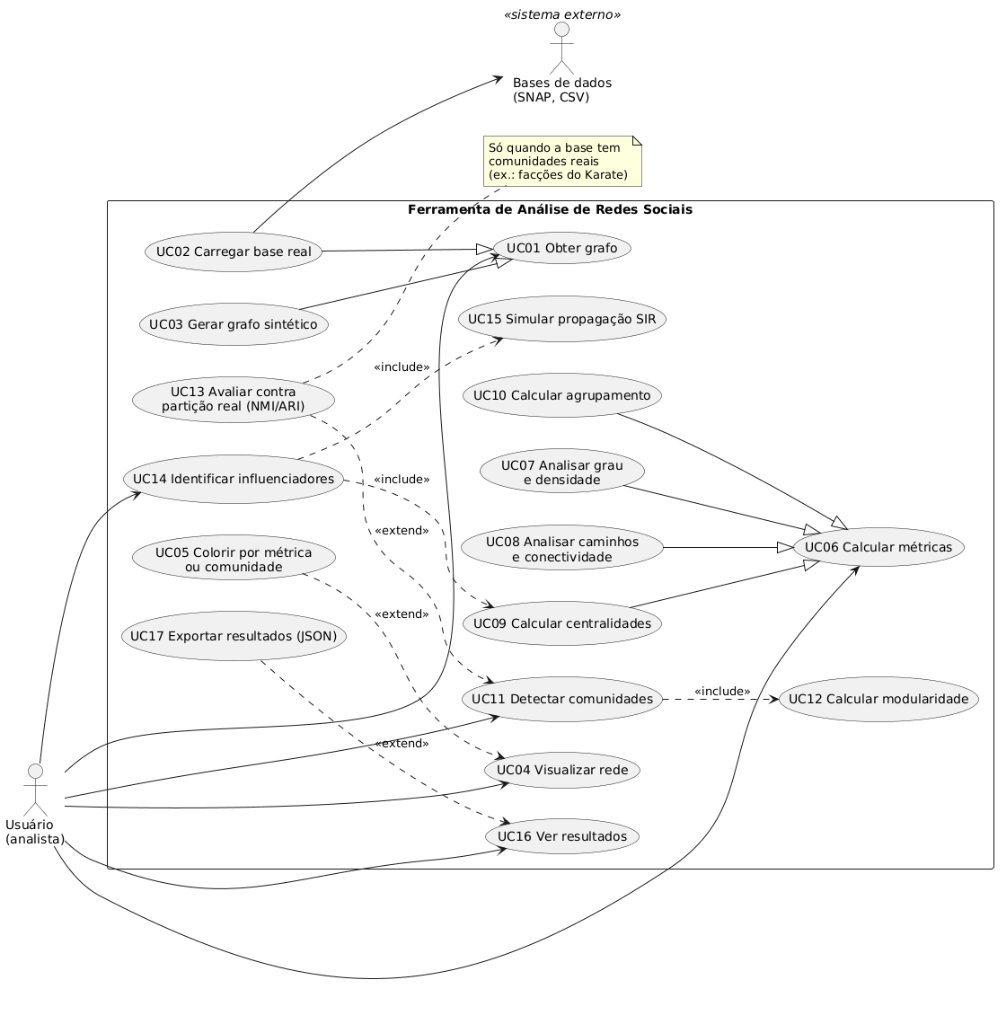
\includegraphics[width=.95\textwidth]{casos_de_uso.jpg}
\caption{Diagrama de casos de uso da ferramenta.}
\label{fig:casos}
\end{figure}

\pendente{Kaio: esboço das seis telas da interface (visão geral, rede, centralidades,
comunidades, influenciadores e desempenho).}
